\section{Lezione del 27/04/2018}

\subsection{Red-Black Trees}

I \emph{Red-Black Trees} sono ABR i cui nodi hanno un campo \emph{colore} $x.col$, che può essere:
\begin{itemize}[noitemsep]
    \item \textbf{R} per il rosso;
    \item \textbf{B} per il nero.
\end{itemize}

\paragraph{Accorgimento} $\const{nil}$ sarà in realtà un nodo,
$T.nil$, con $T.nil.col = B$.

\paragraph{Caratteristiche} \emph{RB-tree} è in realtà un ABR tale che:
\begin{enumerate}[label=($\arabic*$)]
    \item Ogni nodo $x$ ha $x.col \in \{R,B\}$;
    \item La radice $root$ ha $root.col = B$;
    \item Le foglie ($T.nil$) sono $B$;
    \item Se $x$ è $R$, i figli sono $B$;
    \item Per ogni nodo $x$, ogni cammino da $x$ a una qualsiasi delle foglie
    ha lo stesso numero di nodi $B$ (calcolato con $bh(x)$).
\end{enumerate} 

\begin{figure}[hbt]
    \centering
    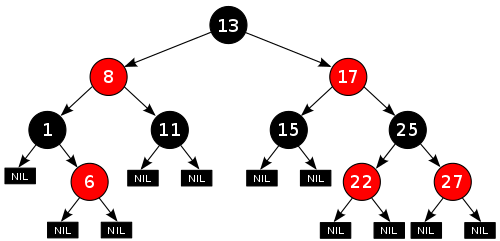
\includegraphics[width=\textwidth]{img/rb-tree-ex.png}
    \caption{Esempio di un RB-tree.}
\end{figure}
\pagebreak

È possibile notare che: 
\begin{itemize}
    \item In caso non ci fossero nodi rossi, avremo un albero
    perfettamente bilanciato;
    \item In ogni cammino, il \verb|#| di nodi \textbf{B} è almeno la
    metà del \verb|#| dei nodi \textbf{R}
\end{itemize}

\paragraph{Osservazione} Se $T$ è un \emph{RB-tree} con $n$ nodi interni ($\neq \const{nil}$)
e $h$ altezza, allora vale
$$h \leq 2 \log (n + 1)$$

\subparagraph{Dimostrazione} Consideriamo 
$$n_x \geq 2^{bh(x)} - 1$$
La dimostrazione è per induzione su $h_x$ (altezza del sotto-albero radicato in $x$).

\begin{description}
    \item[$(h_x = 1)$] Allora ho solo 
    $T.nil \Rightarrow n_x = 0 = 2^0 - 1 \qquad (2^0 \text{ con } 0 = bh(x))$
    \item[$(h_x > 1)$] Consideriamo $x$ radice. $x$ ha due figli, $x_1$ e $x_2$.\par
    Sicuramente vale $h_1,h_2 < h$. Per ipotesi induttiva, valgono:
    $$n_{x_1} \geq 2^{bh(x_1)} - 1$$
    $$n_{x_2} \geq 2^{bh(x_2)} - 1$$
    \begin{align*}
        n_x & = n_{x_1} + n_{x_2} + 1 \\
        & \geq 2^{bh(x_1)} + 2^{bh(x_2)} - 1 \\
        & \geq 2 \cdot 2^{bh(x)-1} - 1 = 2^{bh(x)} - 1 \\
        & \qquad (\text{valgono } bh(x_1) \geq bh(x)-1, \ bh(x_2) \geq bh(x)-1) \\
        \text{Comples}&\text{sivamente}\\
        n & = n_{root} \geq 2^{bh(root)} - 1
    \end{align*}
    Essendo $bh(root) \geq \frac{h}{2}$, posso ottenere
    \begin{align*}
        n_{root} & \geq 2^{bh(root)} - 1 \\
        & 2^{\frac{h}{2}} - 1 \\
        \Rightarrow \ & 2^{\frac{h}{2}} \leq n + 1 \\
        & \frac{h}{2} \leq \log_2(n+1) \Rightarrow h \leq 2 \log_2(n+1) 
    \end{align*}
\end{description}

\subsubsection{Complessità algoritmi RB-Trees}
\texttt{Search, Succ, Min, Pred, Max} hanno un costo di $O(h) = O(\log n)$